\documentclass{article}
%\documentclass[journal,transmag]{IEEEtran}
%\documentclass[10pt, conference]{IEEEtran}
\usepackage{amsmath}
\usepackage{graphicx}
%\usepackage{listings}
%\usepackage{circuitikz}
\usepackage{lscape}
\usepackage{ulem}
\usepackage{float}


\usepackage[scale=0.8]{geometry}
\begin{document}

\title{E6312: Problem Set 4}
\author{Miles Sherman}
\date{\today}
\maketitle

\section{Bullet Point 1}
INSERT SCAN HERE
%\begin{figure}[H]
%\centering
%\includegraphics[width=6in]{1_1}
%\caption{Hand-Written Work for Problem 1.1}
%\label{1_1}
%\end{figure}

\section{Bullet Point 2}
INSERT SCAN HERE

To build the folded cascade OTA, I began by sizing transistors M0, M1, and M2 (see figure \ref{b2_schem} for instance names). Because I want $160\mu A$ through transistor M9 and that transistor is sized with $W = 42\mu m$ and I want $320\mu A$ through transistor M2, I sized M2 at $84\mu A$. For the sake of convenience, I decided to use a $320\mu A$ current source so I sized transistors M0 and M1 at $84\mu A$ as well. In addition, because I will eventually put this circuit into feedback and I would like my output to be close to mid-rail, I set $V_{cm} = 800mV$ which is close to the ceiling of input voltage. This is an acceptable value because the small signal input will never be above 1V.

To bias $V_{b1}$, $V_{b2}$, and $V_{b3}$ I utilized two branches of self-biasing current mirrors (see Figure \ref{b2_schem}). The first branch, which consists of one PMOS and four NMOS transistors, serves a number of purposes. The PFET (M21) mirrors current from M0 and cuts it in half (sized $42\mu A$). The four NMOS receive the $~160\mu A$ of current and are sized as follows. M28 will have half the current of M14 and its gate voltage will bias $V_{b1}$ so it must be half the width of M14, $10.5\mu m$. M29 will have the same current as M13 and its gate voltage will bias $V_{b2}$ so it must be the same width as M13, $10.5\mu A$. M27 will also take the same width as M29 and M28. M20 will take one third of that width. Using a very similar methodology, I built the second self-biasing current mirror branch but this time mirroring the current with an NMOS and receiving the current with four PMOS transistors. M31 mirrors the current of $160\mu A$ so it is sized the same as M28. M44, M45, and M40 will all have the same current as M10 and the gate of M45 will bias $V_{b3}$ so they are all sized the same as M10 at $42\mu A$. M4 is sized one third of that. As can be seen in Figure \ref{b2_dcop}, the biasing is successful.

\begin{figure}[H]
\centering
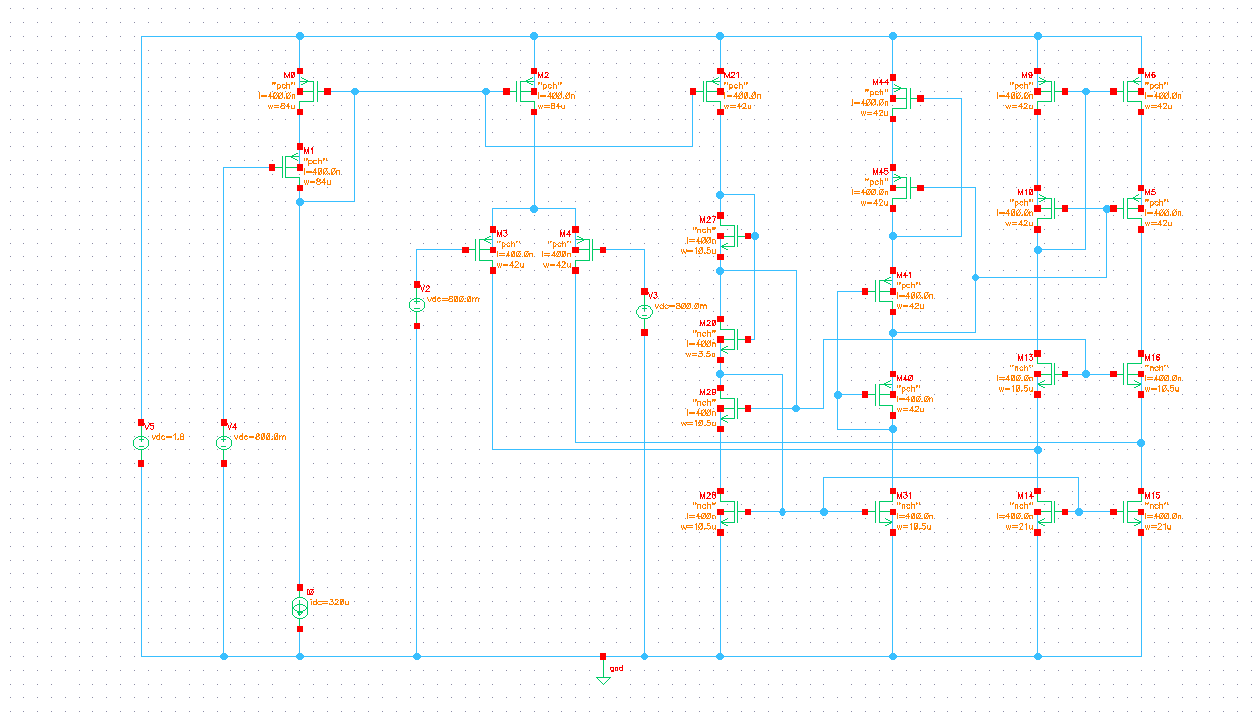
\includegraphics[width=6in]{bullet2_schem.png}
\caption{Schematic Diagram for the Folded Cascode OTA with Associated Biasing Circuitry}
\label{b2_schem}
\end{figure}

\begin{figure}[H]
\centering
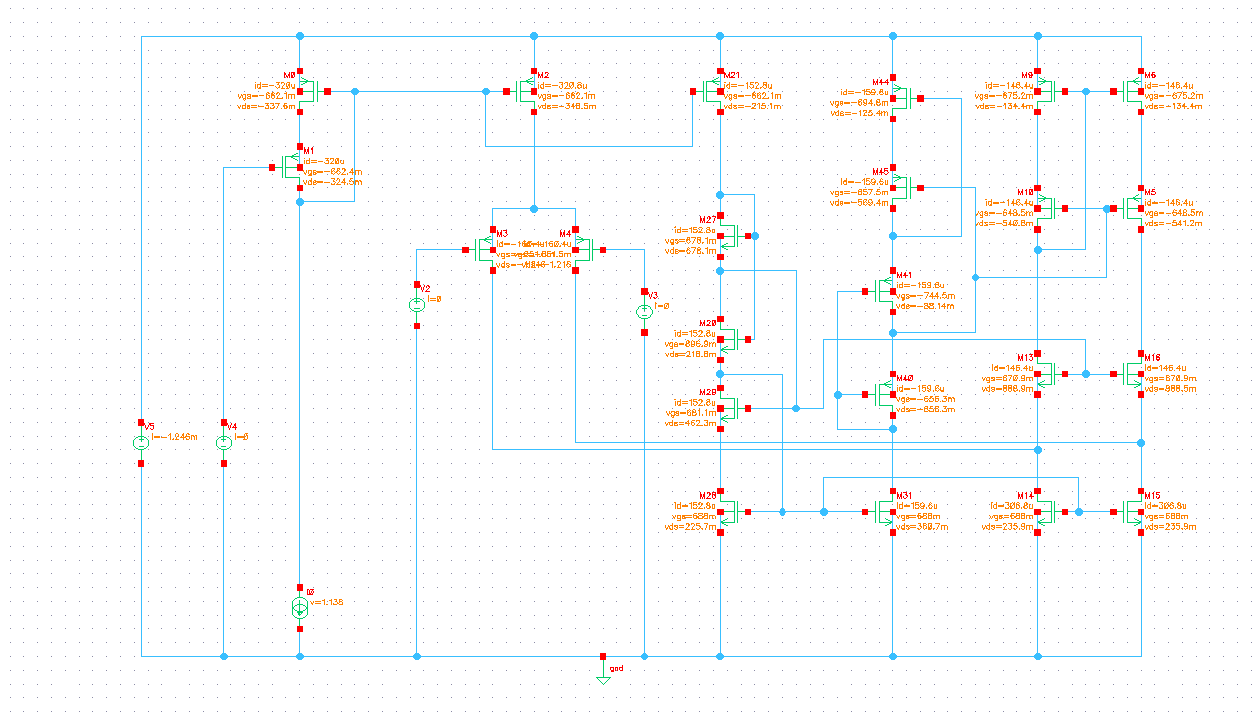
\includegraphics[width=6in]{bullet2_dcop.png}
\caption{Schematic Diagram for the Folded Cascode OTA with Annotated DC Operating Point Values}
\label{b2_dcop}
\end{figure}
\newpage

\section{Bullet Point 3}
I performed a DC sweep of $V_{out-OL}$ against $V_{in-OTA}$ with the OTA in stand alone and the expected transfer function for a differential amplifier is attained (see Figure \ref{b3}).

\begin{figure}[H]
\centering
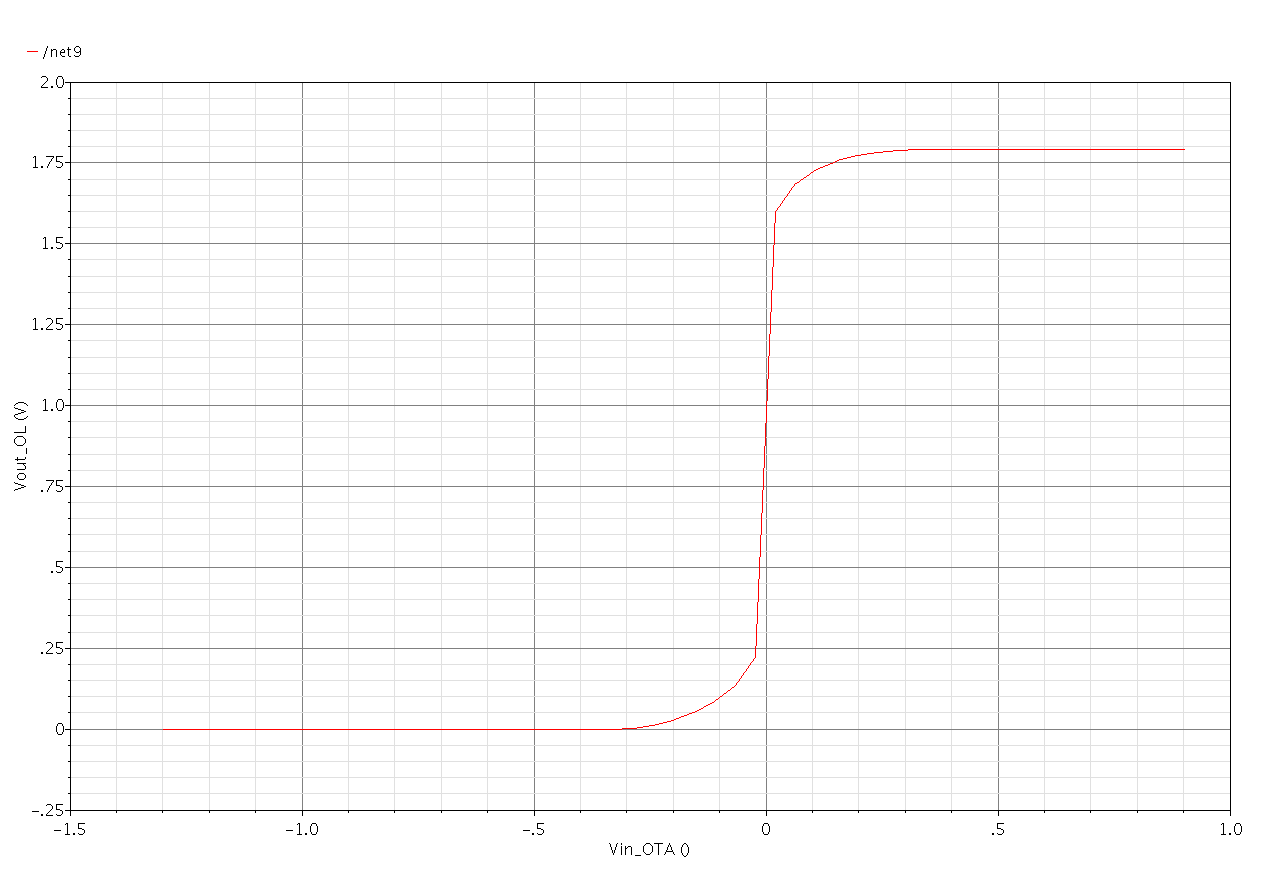
\includegraphics[width=6in]{bullet3.png}
\caption{Voltage Transfer Characteristic for the Folded Cascode OTA in Stand Alone}
\label{b3}
\end{figure}
\newpage

\section{Bullet Point 4}
I applied a small-signal differential input as well as some DC feedback circuitry in order to simulate the open loop gain. Because the open loop gain does not consider small signal feedback, I wanted to build a  circuit that would block all AC feedback. However, I wanted to use this feedback to bias $V_{cm}$. To do this I implemented an RC lowpass filter with a negligible cutoff voltage as can be seen in Figure \ref{b4_schem}. I performed an AC simulation of the open loop gain of the circuit (see Figure \ref{b4_bode}) and was able to attain $A(s) = 485.40\frac{V}{V} = 53.39dB$. Please note that since transistor M44 does not directly affect the biasing, I was able to reduce its size to $~16\mu A$ and optimize my gain.

From the phase plot of my optimized open loop circuit (Figure \ref{b4_bode_opt}), I estimate that there are poles at $~227kHz$ and $471MHz$ and a zero at 945MHz. I estimate the gain-bandwidth product (taken at -3dB from the maximum gain) to be $~72.2MHz$.

\begin{figure}[H]
\centering
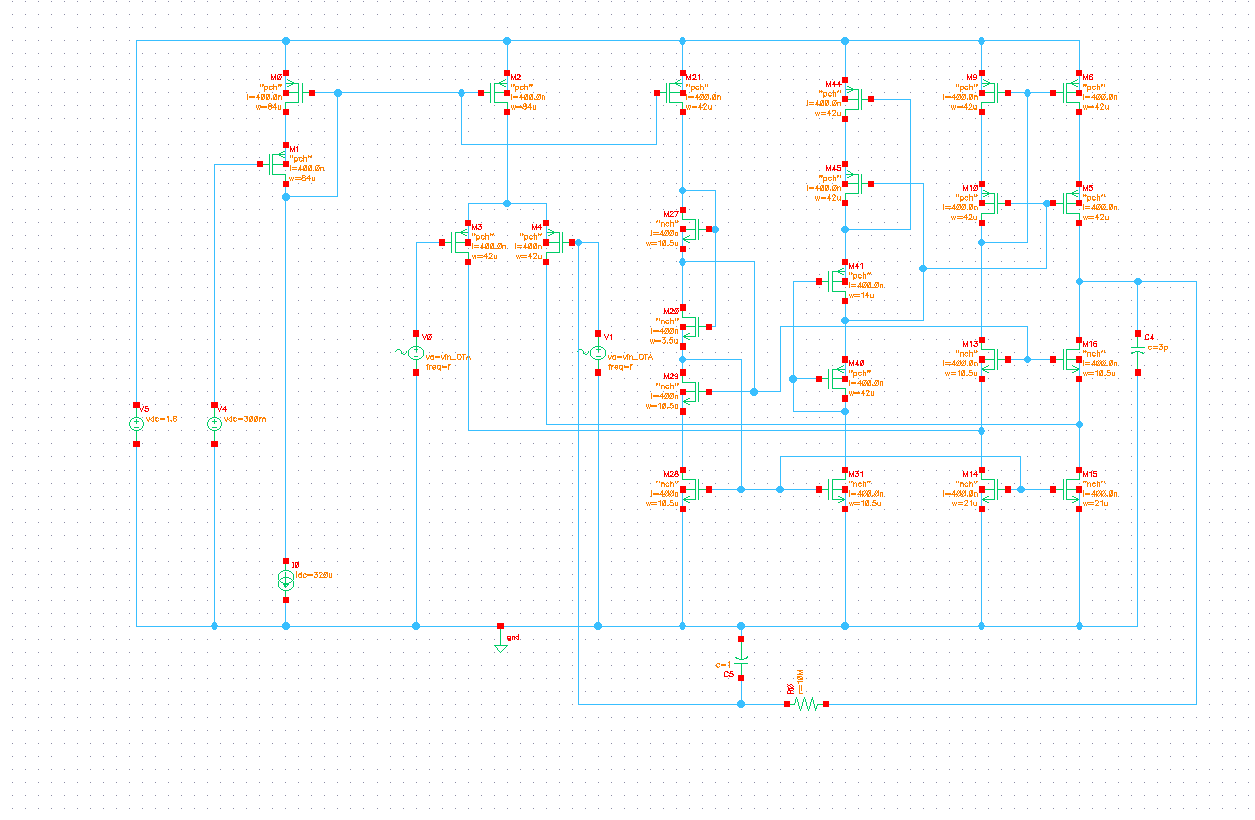
\includegraphics[width=7in]{bullet4_schem.png}
\caption{Schematic Diagram for the Folded Cascode OTA for Open Loop Gain Simulation}
\label{b4_schem}
\end{figure}

\begin{figure}[H]
\centering
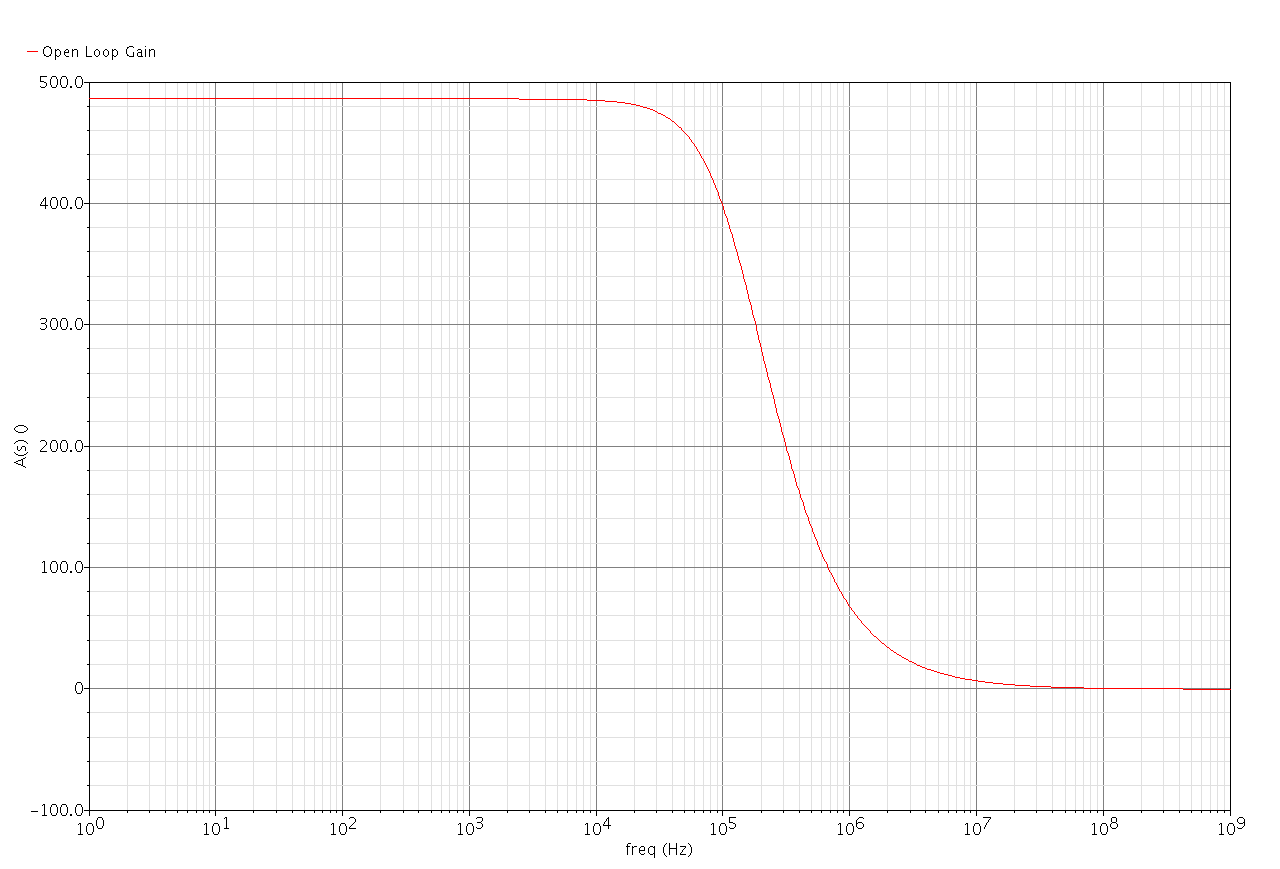
\includegraphics[width=7in]{bullet4_bode.png}
\caption{Bode Plot of the Open Loop Gain of the OTA}
\label{b4_bode}
\end{figure}
\newpage

\section{Bullet Point 5}
INSERT SCAN HERE

\section{Bullet Point 6}


\end{document}
